\documentclass{beamer}
\usetheme{Madrid}
\usecolortheme{default}

% Remove navigation symbols
\beamertemplatenavigationsymbolsempty

% Set poster size
\setbeamersize{text margin left=1cm,text margin right=1cm}

% Title slide
\title{Music-Reactive RGB LEDs Circuit}
\author{Naveed Ahmad \and Muhammad Kamil Khan \and Sharjeel Qureshi}
\date{}

\begin{document}

\begin{frame}[plain]
  \titlepage
\end{frame}

\begin{frame}[t]
  \frametitle{Music-Reactive RGB LEDs Circuit}
  \begin{center}
    \LARGE Presented By \\
    Naveed Ahmad, Muhammad Kamil Khan, Sharjeel Qureshi
  \end{center}

  \vspace{0.5cm}

  \textbf{Introduction:}
  A music-reactive RGB LED circuit combines RGB LEDs and audio input to produce captivating light displays that synchronize with music. The LEDs respond to sound levels and frequencies, creating dynamic lighting effects.

  \vspace{0.5cm}

  \textbf{Components:}
  \begin{itemize}
    \item Mic
    \item NPN Transistor (e.g., BC547)
    \item Resistors: 10k (2), 1k (4), 1M (1)
    \item Ceramic Capacitor: 100nF
    \item RGB LEDs
    \item 9V Battery
    \item Breadboard and wires
  \end{itemize}

  \vspace{0.5cm}

  \textbf{Working:}
  \begin{enumerate}
    \item Mic captures sound signals and converts them into voltage.
    \item High-pass filter removes unwanted noise.
    \item NPN transistor amplifies filtered signals.
    \item Amplified signals trigger transistors, lighting up corresponding LEDs based on sound patterns.
  \end{enumerate}

  \vspace{0.5cm}

  \begin{center}
    \textbf{Schematic Diagram}
    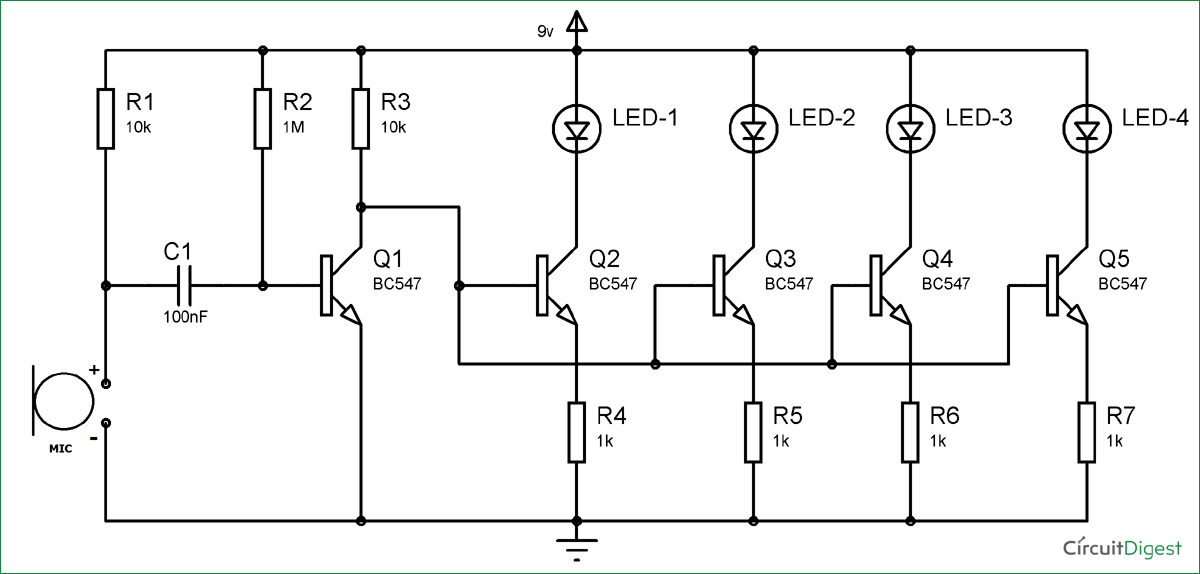
\includegraphics[scale=0.7]{image1.png}
  \end{center}
\end{frame}

\end{document}

